\section{I$^2$C sběrnice}
\label{sec:i2c-sbernice}

\begin{figure}[H]
   \centering
    \def\svgwidth{0.3\columnwidth}
   \input{images/svg/otopna-soustava/vyrez-i2c-sbernice.pdf_tex}
    \caption[Výřez pro modul I$^2$C sběrnice u centrální jednotky.]{Výřez z obrázku \ref{fig:otopna-soustava-a-elektronika-rez-domu} – modul I$^2$C sběrnice u centrální jednotky.}
    \label{fig:vyrez-i2c-sbernice}
\end{figure}

Na obrázku \ref{fig:vyrez-i2c-sbernice} je výřez části z celkového nákresu (obrázek \ref{fig:otopna-soustava-a-elektronika-rez-domu}) pro modul I$^2$C sběrnici u centrální jednotky. Sběrnice I$^2$C je realizovaná pomocí zakoupeného modulu (obrázek \ref{fig:modul-pca9615-i2c-sbernice}) s~obvodem PCA9615 \cite{vyrobce-pca9615} (blokové schéma je v příloze \ref{fig:blokove-schema-pca9615-i2c-sbernice}) do firmy  NXP Semiconductors. Vstupní signál SCL a~SDA je veden přímo z~centrální jednotky na vstupu obvodu PCA9615, napájení je s 3,3 V logikou. Výstup z PCA9615 je pomocí diferenciální veden. Napájení na této straně je 5 V. Sběrnice je realizovaná pomocí UTP kategorie 5e, výstup z~modulu je realizován pomocí konektoru RJ45. Vzhledem k použití UTP kabelu a diferenciálnímu přenosu je možné dosáhnout velké vzdálenosti sběrnice. Nejdelší bod dosahuje přibližně 30 m, je tedy možné použít I$^2$C sběrnici na vzdálenost, pro kterou není standartě dělána. Použitá frekvence je 100~kHz. Jedná se tedy o plnohodnotnou I$^2$C sběrnici. Důvodem pro zvolení této varianty bylo na základě výběru displeje s I$^2$C sběrnicí (jednoduché a~levné řešení), dále jedná se o klasické zapojení displeje jako by se nalézal v~krátké vzdálenosti od centrální jednotky a není tak nutný převod jako při využít např. RS485 na UART a následně na I$^2$C sběrnici, v neposlední řadě komunikace je definována podle protokolu I$^2$C.  Jeden modul se nalézá na straně centrální jednotky a pak na straně krbů. Napájení 5 V je realizováno pomocí samostatných kabelů, není tedy součástí UTP kabelu. Z důvodu omezení kabeláže je sběrnice realizována v jednom UTP kabelu s 1-Wire sběrnicí, tedy přesněji jsou využity volné vodiče 1,2 pro SCL a~7,~8 pro SDA. Zařízení lze zapojovat jak na straně před PCA9615, tak i~na diferenciální straně, je však výhodné připojené uzly udržet co v~nejkratší vzdálenosti kvůli degradování signálu. Blokové schéma je na obrázku \ref{fig:blokove-schema-pca9615-i2c-sbernice} včetně napojení uzlů. Schéma zapojení modulu v příloze \ref{app:schemata-ostatni}, upraveno z \cite{pca9615-schema-zapojeni}.


Výhodou PCA9615 je automatický výběr směru komunikace, není potřeba externí ovládání. Komunikace je možná až do rychlosti 1 MHz (přibližně pro 3 m), se zvýšenou délkou je však nutné rychlost snížit. Komunikace využívá standardní protokol I$^2$C. Koncová zařízení je možné napájet z různých zdrojů. V neposlední řadě se jedná o jednoduché řešení bez nutných další zařízení na straně Slave, stačí pouze zapojit koncové zařízení s~podporou I$^2$C. Na obrázku \ref{fig:modul-pca9615-transily} jsou pro větší ochranu modulu přidány obousměrné transil diody (SM6T6V8CAY \cite{sm6t6v8cay}) připájené na vstupní piny konektoru RJ45 (obvod sám o sobě poskytuje vstupní ochranu pro ESD). Pro rozbočení I$^2$C sběrnice do jednotlivých pater slouží DPS s konektory RJ45 (schéma viz příloha \ref{app:schemata-ostatni}, obrázky viz příloha \ref{app:rozbocovac-i2c}).

\begin{figure}[H]
\centering
\begin{subfigure}{.5\textwidth}
    \centering
    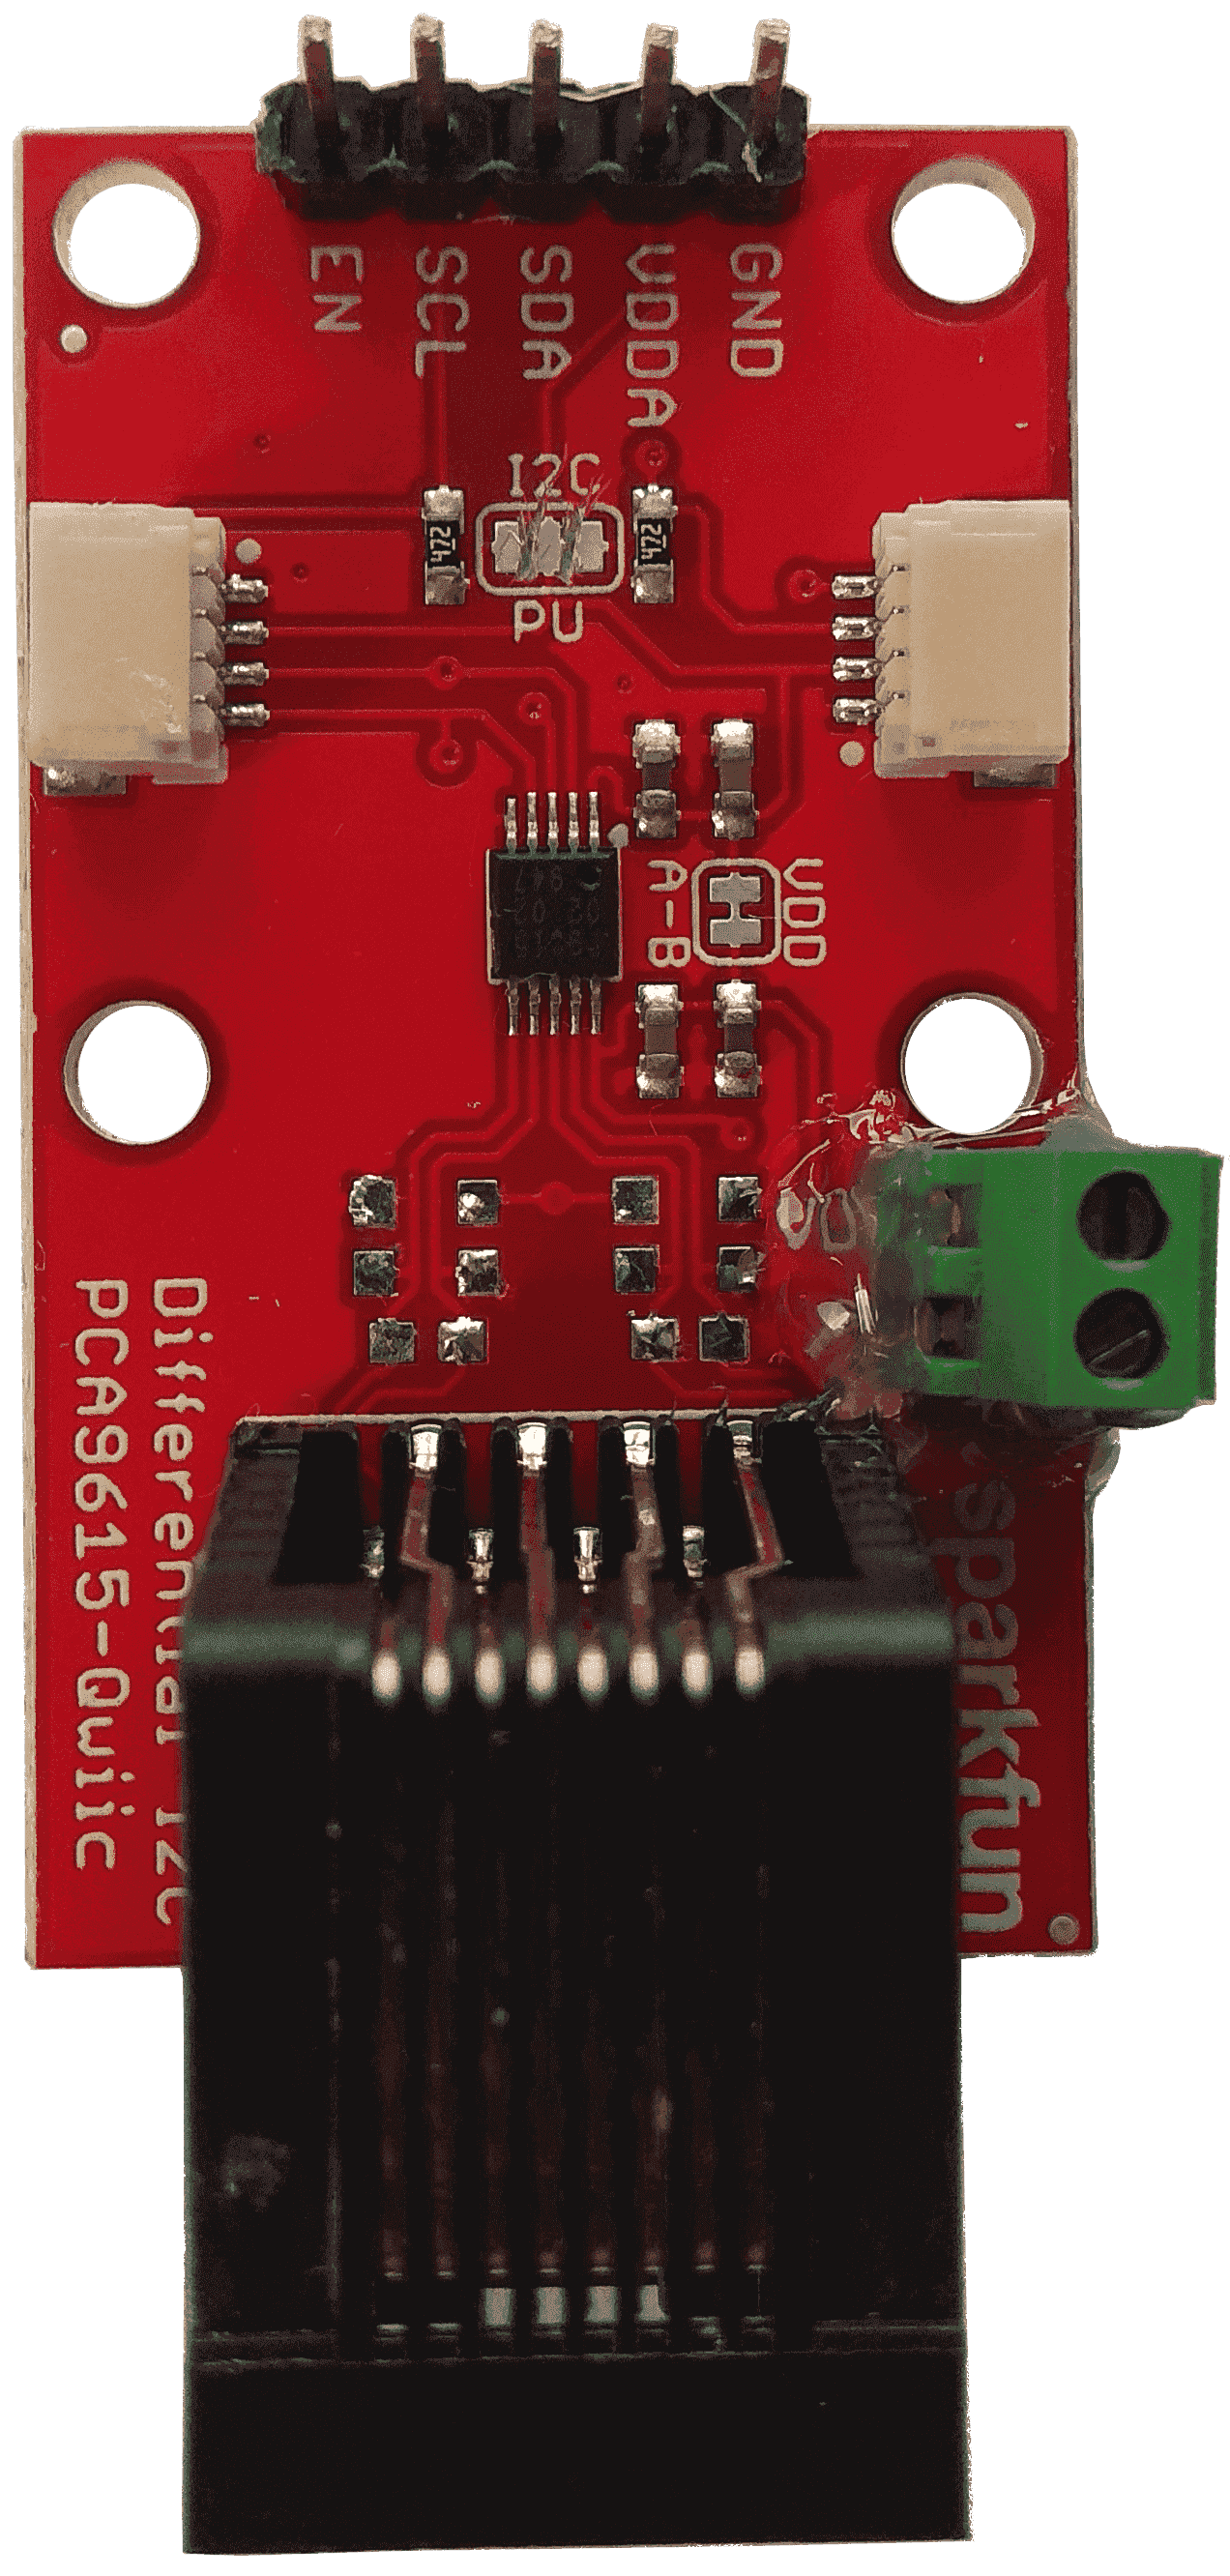
\includegraphics[width=0.53\textwidth]{images/krb/modul-pca9615-i2c-sbernice.png}
    \caption{Vrchní strana.}
    \label{fig:modul-pca9615-i2c-sbernice}
\end{subfigure}%
\begin{subfigure}{.5\textwidth}
    \centering
    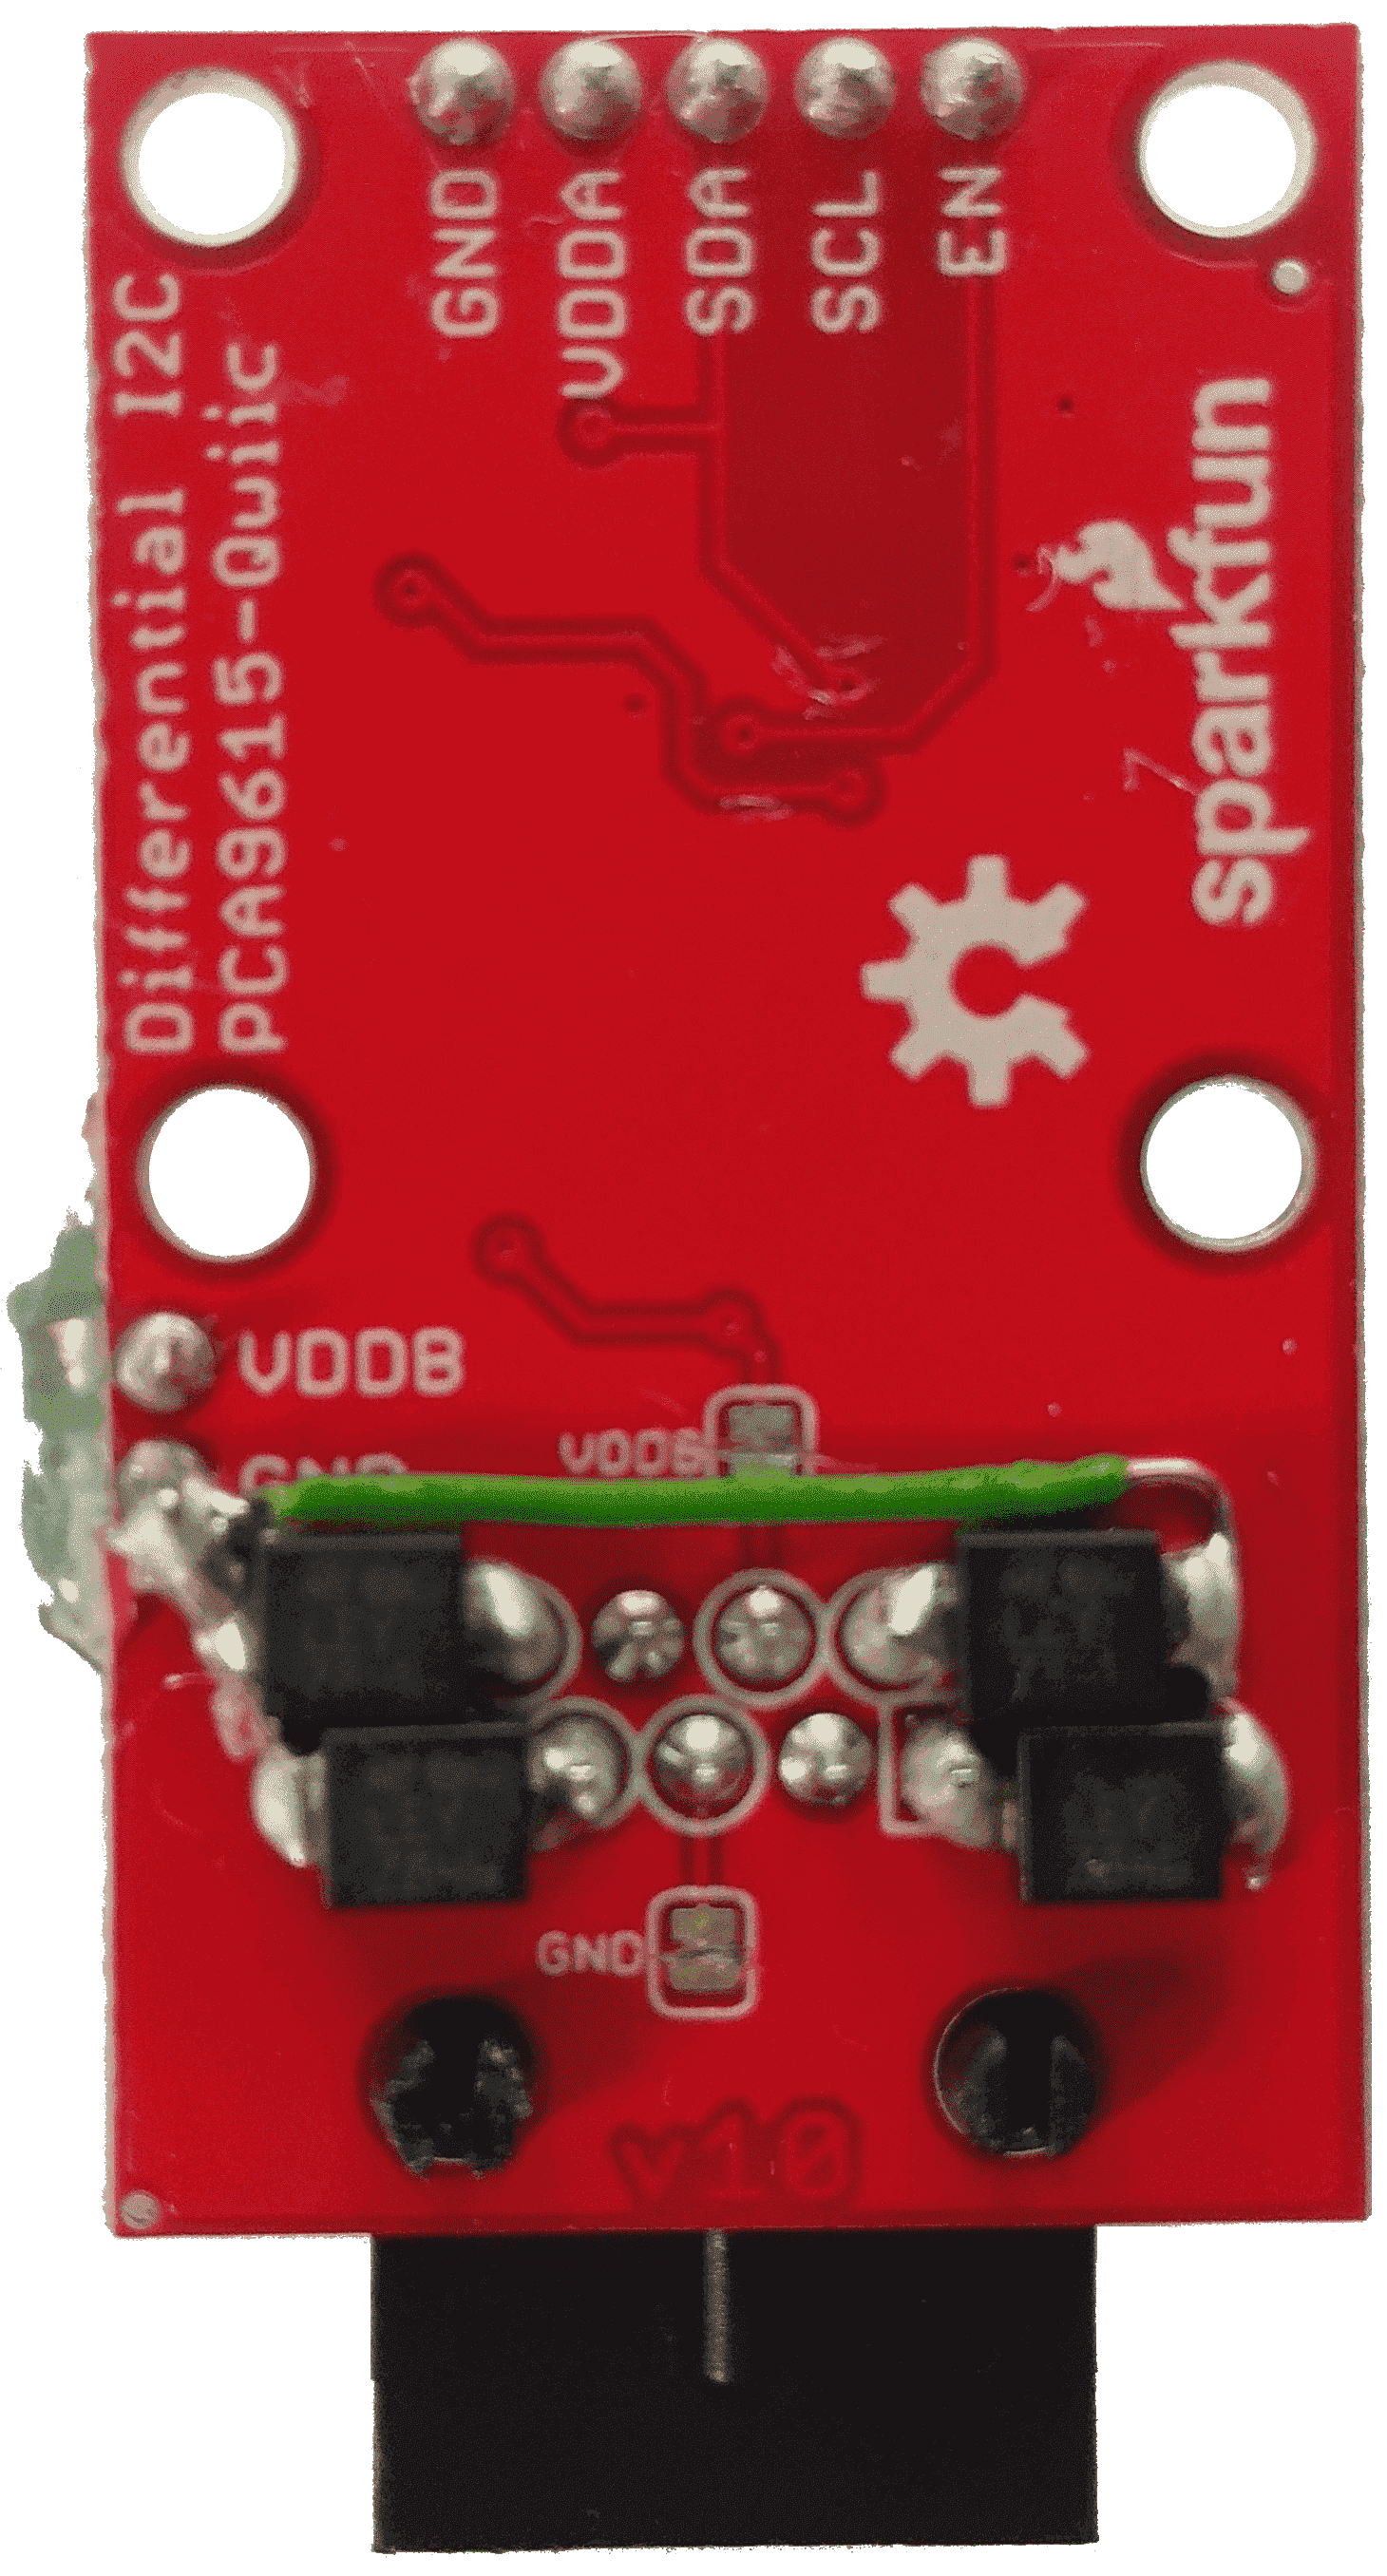
\includegraphics[width=0.6\textwidth]{images/krb/modul-pca9615-transily.png}
    \caption{Spodní strana s ochrannými transily.}
    \label{fig:modul-pca9615-transily}
\end{subfigure}
\caption{Modul s obvodem PCA9615.}
\label{fig:modul-pca9615}
\end{figure}